\chapter{Reduction to Hessenberg or Tridiagonal Form} 
We now describe the first of the two computational phases outlined in the previous chapter: reduction of a full matrix to Hessenberg form by a sequence of unitary similarity transformations. If the origional matrix is hermitian, the result is tridiagonal. 

\section{A Bad Idea}
To compute the Schur factorization $A = QT Q^* $, a natural first idea might be to attempt direct triangularization by Householder reflectors. We consider the following case. As usual, entries that are changed at each step are written in boldface:
%────────────────────────────────────────
\begin{figure}[H]
    \centering
    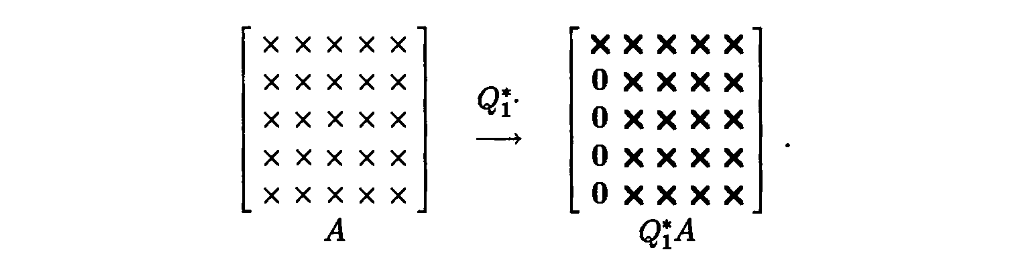
\includegraphics[width=0.8\textwidth]{figures/26-1.png}
\end{figure}
%────────────────────────────────────────   
Unfortunately, to complete the similarity transformation, we must also multiply by $Q_1$ on the right of $A$: 
%────────────────────────────────────────
\begin{figure}[H]
    \centering
    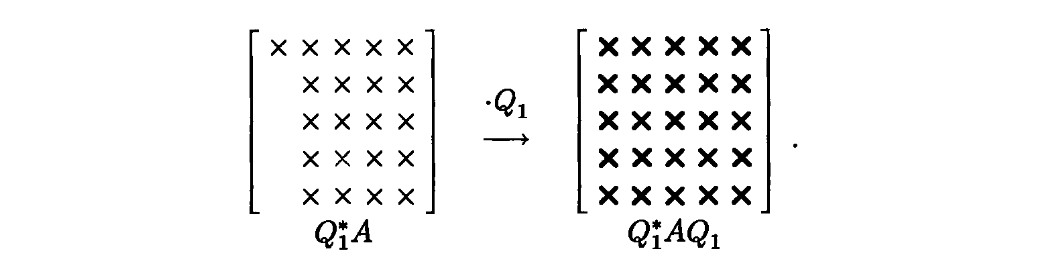
\includegraphics[width=0.8\textwidth]{figures/26-2.png}
\end{figure}
%────────────────────────────────────────
This has the effect of replacing each column of the matrix by a linear combination  of all the columns. The result is that the zeros that were previously introduced are destroyed; we are no better off than when we started.  

Of course, this is doomed to fail, since we know no finite process can reveal the eigenvalues of $A$ exactly. Curiously, this too-simple strategy, which appears futile as we have discussed it, does have the effect, typically, of reducing the size of the entries below the diagonal, even if it does not make them zero.  

\section{A Good Idea}
The right strategy for introducing zeros in Phase 1 is to be less ambitious and operate on fewer entries of the matrix. We shall only conquer territory we are sure we can defend. 

At the first step, we select a Householder reflector $Q_1^*$ that leaves the first row unchanged. When it is multiplied on the left of $A$, it forms linear combinations of only rows $2,\ldots ,m$ to introduce zeros into row $3,\ldots ,m$ of the first column. Then, when $Q_1$ is multiplied on the right of $Q_1^*A$, it leaves the first column unchanged. 
%────────────────────────────────────────
\begin{figure}[H]
    \centering
    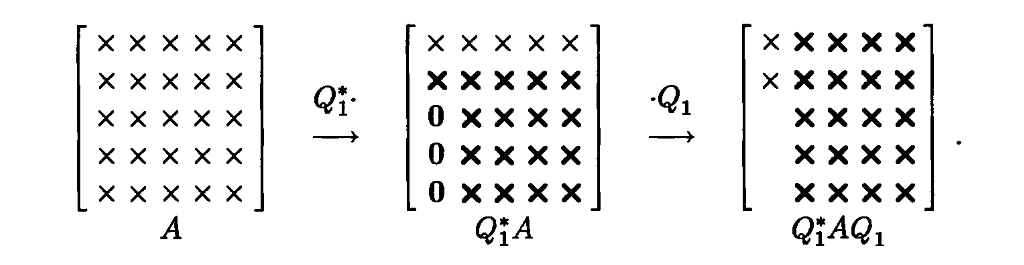
\includegraphics[width=0.8\textwidth]{figures/26-3.png}
\end{figure}
%────────────────────────────────────────
This idea is repeated to introduce zeros into subsequent columns. Then we can also find a second $Q_2$ to change the second column: 
%────────────────────────────────────────
\begin{figure}[H]
    \centering
    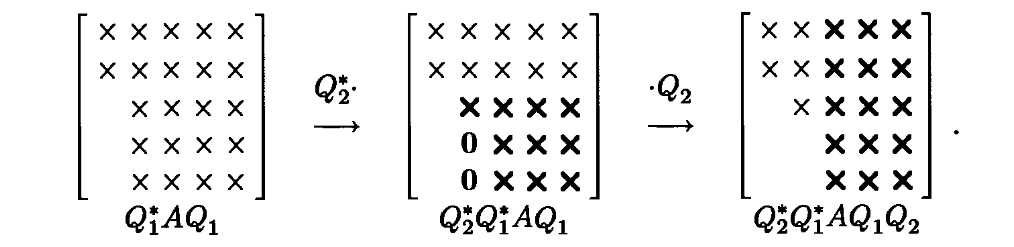
\includegraphics[width=0.8\textwidth]{figures/26-4.png}
\end{figure}
%────────────────────────────────────────
After  repeating this process $m-2$ times, we have a product in Hessenberg form, as desired: 
%────────────────────────────────────────
\begin{figure}[H]
    \centering
    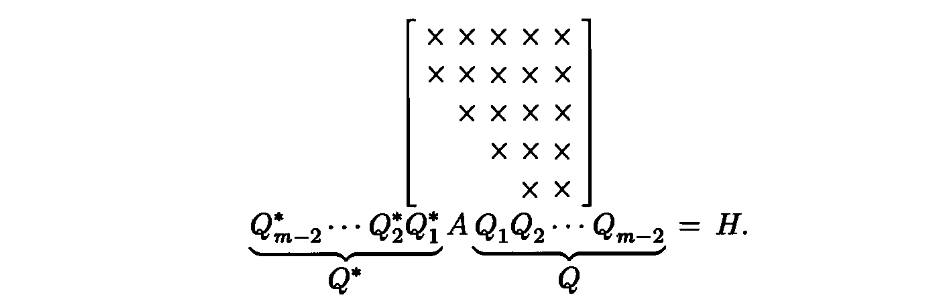
\includegraphics[width=0.8\textwidth]{figures/26-5.png}
\end{figure}
%────────────────────────────────────────
The algorithm is formulated below.  

\begin{algorithm}[H]
    \caption{Householder Reduction to Hessenberg Form}
    \label{Algo 26.1}
    \For{$k=1$ \KwTo $m-2$}{
        $x = A_{k+1:m, k}$\; 
        $v_k = \sign(x_1) \|x\|_2 e_1 + x$\; 
        $v_k = v_k/ \|v_k\|_2$\; 
        $A_{k+1:m, k:m} = A_{k+1:m,k:m} - 2v_k (v_k^* A_{k+1:m, k:m})$\; 
        $A_{1:m, k+1:m} = A_{1:m, k+1:m} - 2(A_{1:m, k+1:m} v_k)v_k^*$\;
    }
\end{algorithm}


\section{Operation Count}
The number of operations required by Algo~\ref{Algo 26.1} can be counted with the same geometric reasoning we have used before. The rule of thumb is that unitary operations require four flops for reach element operated upon. 

The work is dominated by the two updates of submatrices of $A$. The first loop applies a Householder reflector on the left of the matrix. The $k$ th such reflector operates on the last $m-k$ rows. Note that arithmetic has to be perfomed only on the last $m-k+1$ entries of each row. The picture is as follows: 
%────────────────────────────────────────
\begin{figure}[H]
    \centering
    
\includegraphics[width=0.8\textwidth]{figures/26-6.png}
\end{figure}
%────────────────────────────────────────
As $m\to \infty$, the volume converges to $ \frac{1}{3}m^3 $. At four flops per element, the amount of work in this loop is $\sim \frac{4}{3}m^3$ flops. 

The second inner loop applies a Householder reflector on the right of the matrix. At the $k$th step, the reflector operates by forming linear combination of the last $m-k$ columns. This loop involves more work than the first one because there are no zeros that can be ignored. Arithmetic must be performed on all of the $m$ entries of each of the columns operated upon. A total of $m(m-k)$ entries for a single value of $k$. The picture looks like this: 

%────────────────────────────────────────
\begin{figure}[H]
    \centering
    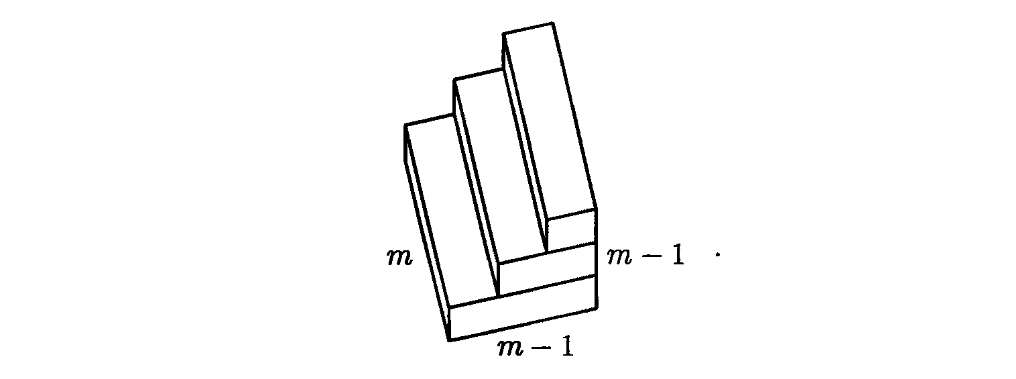
\includegraphics[width=0.8\textwidth]{figures/26-7.png}
\end{figure}
%────────────────────────────────────────
The volume converges as $m\to \infty$ to $\frac{1}{2}m^3$, so, at four flops per element, this second loop requires $\sim 2m^3$ flops. 


%────────────────────────────────────────
\begin{theorem}
\label{thm: Work Hessenberg reduction}
The work for Hessenberg reduction: $\sim \frac{10}{3} m^3$ flops. 
\end{theorem}
%────────────────────────────────────────

\section{The Hermitian Case} 
If $A$ is hermitian, the algorithm will reduced $A$ to tridiagonal form. Since zeros are now introduced in rows as well as columns, additional arithmetic can be avoided by ignoring these additional zeros. Hence, the total amount of arithmetic is reduced to $\frac{8}{3}m^3$. 

However, if we take advantage of both sparsity and symmetry, the toal work can be further reduced by a factor of two. 


%────────────────────────────────────────
\begin{theorem}
\label{thm: Work tridiagonal reduction}
Work for tridiagonal reduction: $ \sim \frac{4}{3}m^3 $ flops. 
\end{theorem}
%────────────────────────────────────────

\section{Stability}
Like the Householder algorithm for QR factorization, the algorithm just described is backward stable. Let $\tilde H$ be the actual Hessenberg matrix computed in floating arithmetic, and let $\tilde Q$, as before, be the exactly unitary matrix corresponding to the reflection vectors $\tilde v_k$ computed in floating point arithmetic. We have 


%────────────────────────────────────────
\begin{theorem}
[Backstab of Hessenberg reduction]
\label{thm: Backstab of Hessenberg reduction}
Let the Hessenberg reduction $A = QHQ^* $ of a matrix $A\in \CC^{m\times m}$ be computed by Algo~\ref{Algo 26.1} on a computer satifying the axioms \eqref{eq: fler} and \eqref{eq:flop}, and let the computed factors $\tilde Q$ and $ \tilde H $ be defiend as indicated above. Then we have 
\begin{equation}
\label{eq: backstab of Hessenberg}
    \tilde Q \tilde H \tilde Q ^*  = A + \delta A, \quad \frac{\|\delta A\|}{\|A\|} = O(\mep)
\end{equation}
for some $ \delta A \in \CC^{m\times m} $. 

\end{theorem}
%────────────────────────────────────────
